% Copyright 2004 by Till Tantau <tantau@users.sourceforge.net>.
%
% In principle, this file can be redistributed and/or modified under
% the terms of the GNU Public License, version 2.
%
% However, this file is supposed to be a template to be modified
% for your own needs. For this reason, if you use this file as a
% template and not specifically distribute it as part of a another
% package/program, I grant the extra permission to freely copy and
% modify this file as you see fit and even to delete this copyright
% notice. 

\documentclass{beamer}

% There are many different themes available for Beamer. A comprehensive
% list with examples is given here:
% http://deic.uab.es/~iblanes/beamer_gallery/index_by_theme.html
% You can uncomment the themes below if you would like to use a different
% one:
%\usetheme{AnnArbor}
%\usetheme{Antibes}
%\usetheme{Bergen}
%\usetheme{Berkeley}
%\usetheme{Berlin}
%\usetheme{Boadilla}
%\usetheme{boxes}
%\usetheme{CambridgeUS}
%\usetheme{Copenhagen}
%\usetheme{Darmstadt}
%\usetheme{default}
%\usetheme{Frankfurt}
%\usetheme{Goettingen}
%\usetheme{Hannover}
%\usetheme{Ilmenau}
%\usetheme{JuanLesPins}
%\usetheme{Luebeck}
\usetheme{Madrid}
%\usetheme{metropolis}
%\usetheme{Malmoe}
%\usetheme{Marburg}
%\usetheme{Montpellier}
%\usetheme{PaloAlto}
%\usetheme{Pittsburgh}
%\usetheme{Rochester}
%\usetheme{Singapore}
%\usetheme{Szeged}
%\usetheme{Warsaw}

%\usepackage{graphicx}
%\usepackage{placeins}
%%\usepackage{sidenotes}
%%\usepackage[a4paper,left=24.8mm,top=27.4mm,headsep=2\baselineskip,textwidth=107mm,
%%					marginparsep=8.2mm,marginparwidth=49.4mm,textheight=49\baselineskip,
%%					headheight=\baselineskip]{geometry} % tufte-handout definitions
%\usepackage[a4paper,
%left=22mm,top=27.4mm,
%headsep=2\baselineskip,
%textwidth=107mm, %110mm
%marginparsep=6.0mm, %4.0mm
%marginparwidth=70mm, %70mm
%textheight=52\baselineskip,
%headheight=\baselineskip]{geometry} % tufte-handout definitions

%=======Fonts and Language [XelateX only]=====
\usepackage{fontspec}
\usepackage{float}
\usepackage{morefloats}
\usepackage{polyglossia}
\usepackage{svg}

\setmainlanguage{greek}
\setotherlanguage{english}

\setmainfont{CF Jeckyl}
\newfontfamily\greekfont{CF Jeckyl}
\newfontfamily\greekfontsf{CF Jeckyl}
\newfontfamily\greekfonttt{CF Jeckyl}
%\setmainfont{Liberation Serif}
%\newfontfamily\greekfont{Liberation Serif}
%\newfontfamily\greekfontsf{Liberation Serif}
%\newfontfamily\greekfonttt{Liberation Serif}

%====Physics and Maths Symbols=============
\usepackage{amsmath}
\usepackage{amssymb}
\usepackage{xparse}
%\usepackage[arrowdel]{physicsrev} %Physics Packge (Revised)
\usepackage[arrowdel]{physics}
\usepackage[version=3]{mhchem} %Chemistry Symbols
\usepackage{wasysym} %Astronomical Symbols

\usepackage{siunitx} %Units
\usepackage{cancel}
\usepackage{multirow}
%=====Graphics=============
\usepackage{graphicx}
%\usepackage{caption}
\usepackage{lipsum, calc, needspace}
%\usepackage{subcaption}
\usepackage{textcomp}
%\usepackage{tikz}
\usepackage{scrextend}
%============================
\newlength\widthw
\setlength{\widthw}{\textwidth+\marginparsep+\marginparwidth}


\newlength{\fullwidthlen}
\setlength{\fullwidthlen}{\marginparwidth}
\addtolength{\fullwidthlen}{\marginparsep}

\newenvironment{fullwidth}{%
	\begin{adjustwidth*}{\ifthispageodd{-5cm}{-0cm}}{\ifthispageodd{-0cm}{-5cm}}%
	}{%
	\end{adjustwidth*}%
}

%======Other==============
\usepackage{multirow}
\usepackage{booktabs}
\usepackage{latexsym,graphicx}
\usepackage{todonotes}
%\usepackage{xcolor}
%\usepackage[some]{background}
%\usepackage{wrapfig}
%\usepackage{sidecap}
%\usepackage{lscape}
%\usepackage{rotating}
%\usepackage{geometry}

%===Bibliography======================
\usepackage[backend=biber,style=authoryear,citestyle=authoryear]{biblatex}
%\addbibresource{My Library.bib}

%=========Unit Declaration==========
\DeclareSIUnit \cm {\centi\meter}
\newcommand{\sm}{$M_{\odot}$}

\title{Αριθμητικές προσομοιώσεις νεφών σε γαλαξίες}
\author{Παπαχρήστου Μιχάλης}
%
%\numberwithin{equation}{subsection}
%\setsecnumdepth{chapter}
%\setcounter{secnumdepth}{3}
%\counterwithout{section}{chapter}
%\newcommand{\tabletodo}[3][]{\begin{minipage}{#2}\todo[inline,#1]{#3}\end{minipage}}
\sisetup{retain-unity-mantissa = false,range-phrase=\texttt{ έως },range-units = single,separate-uncertainty = true}

%\title{Presentation Title}

% A subtitle is optional and this may be deleted
%\subtitle{Optional Subtitle}

%\author{F.~Author\inst{1} \and S.~Another\inst{2}}
% - Give the names in the same order as the appear in the paper.
% - Use the \inst{?} command only if the authors have different
%   affiliation.

%\institute[Universities of Somewhere and Elsewhere] % (optional, but mostly needed)
%{
%  \inst{1}%
%  Department of Computer Science\\
%  University of Somewhere
%  \and
%  \inst{2}%
%  Department of Theoretical Philosophy\\
%  University of Elsewhere}
% - Use the \inst command only if there are several affiliations.
% - Keep it simple, no one is interested in your street address.

\date{28 Ιουνίου 2017}
% - Either use conference name or its abbreviation.
% - Not really informative to the audience, more for people (including
%   yourself) who are reading the slides online

%\subject{Theoretical Computer Science}
% This is only inserted into the PDF information catalog. Can be left
% out. 

% If you have a file called "university-logo-filename.xxx", where xxx
% is a graphic format that can be processed by latex or pdflatex,
% resp., then you can add a logo as follows:

% \pgfdeclareimage[height=0.5cm]{university-logo}{university-logo-filename}
% \logo{\pgfuseimage{university-logo}}

% Delete this, if you do not want the table of contents to pop up at
% the beginning of each subsection:
%\AtBeginSubsection[]
%{
%  \begin{frame}<beamer>{Outline}
%    \tableofcontents[currentsection,currentsubsection]
%  \end{frame}
%}

% Let's get started
\begin{document}

\begin{frame}
  \titlepage
\end{frame}

%\begin{frame}{Outline}
%  \tableofcontents
%  % You might wish to add the option [pausesections]
%\end{frame}

% Section and subsections will appear in the presentation overview
% and table of contents.
\section{Μεσοαστρική Ύλη}

%\subsection{First Subsection}

\begin{frame}{Μεσοαστρική Ύλη}{Τι υπάρχει μεταξύ των αστέρων?}
	Στο μεσοαστρικό χώρο έχουμε μια τεράστια ποσότητα ύλης υπό τη μορφή αερίου (99\%) και σκόνης (1\%). Στο γαλαξία μας η συνολική της μάζα είναι της τάξης των \SI{1e9}{ M_{\odot}}, ενώ η πυκνότητα της κυμαίνεται από \SIrange{1e-4}{1e6}{cm^{-3}}.
\begin{center}
	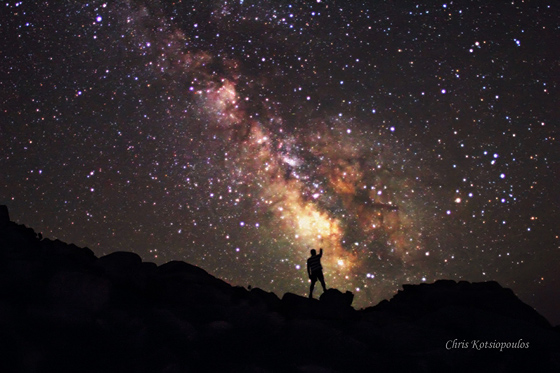
\includegraphics[width=0.8\linewidth]{Images/NightSkyPhotography04}
\end{center}
\end{frame}

\begin{frame}{Μεσοαστρικό αέριο}%{Φυσικά Χαρακτηριστικά}
\begin{center}
	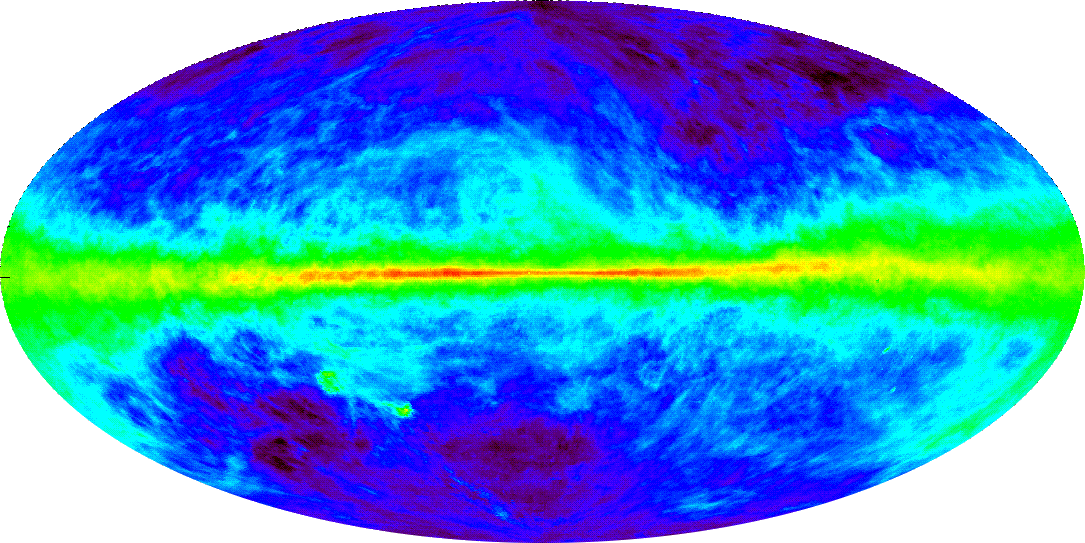
\includegraphics[width=1\linewidth]{../Document/Images/21}
\end{center}


		\begin{itemize}
			\item{(90\%) Υδρογόνο  \ce{(H)}, \ce{(HII)}, \ce{(H2)}}	
			\item{(9\%) Ήλιο }	
			\item{(1\%) Βαρύτερα στοιχεία  (\ce{C},\ce{O},\ce{Ne},\ce{Mg},\ce{Fe}, κ.α.) και μόρια (\ce{CO},\ce{CS}, κ.α.).}
		\end{itemize}

%		\begin{itemize}
%		\item{Υδρογόνο (\ce{HI}, \ce{HII}, \ce{H2} )}
%		\item{Ήλιο (\ce{HeI}, \ce{HeII})}
%		\item{Βαρύτερα στοιχεία (\ce{C}, \ce{O}, \ce{Ne}, \ce{Mg}, \ce{Fe})}
%		\item{Μόρια (\ce{CO}, \ce{CS}, και πολυπλοκότερα PAH)}
%		\item{Σκόνη}
%	\end{itemize}
\end{frame}

\begin{frame}{Μεσοαστρική Σκόνη}%{Χημική Σύσταση}
		\begin{itemize}
		\item{Αποτελείται κυρίως από άνθρακα και πυρίτιο σε ενώσεις με Υδρογόνο, Οξυγόνο, Μαγνήσιο και Σίδηρο}
			\item{Tο μέγεθος των κόκκων της σκόνης κυμαίνεται από \SI{0.01}{\micro\meter} έως \SI{1}{\micro\meter} ακολουθώντας μια κατανομή δύναμης όπου τα μικρότερα μεγέθη είναι πολυπληθέστερα από τα μεγαλύτερα.}
	\end{itemize}
	\begin{columns}
		\column{0.5\textwidth}
		\begin{center}
			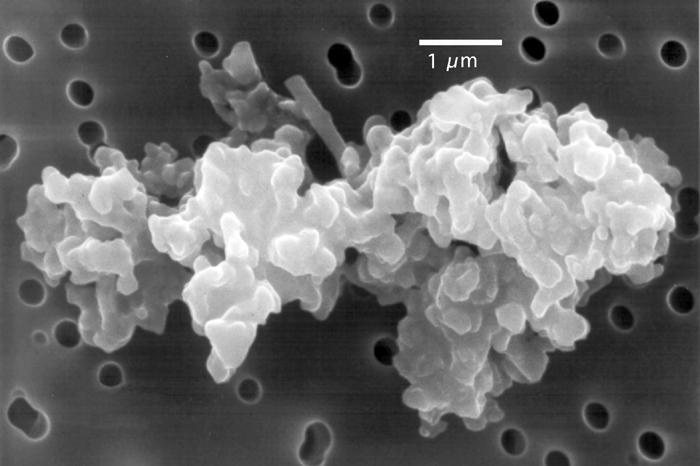
\includegraphics[width=1\linewidth]{Images/Porous_chondriteIDP}
		\end{center}
		
		\column{0.5\textwidth}
		\begin{itemize}
		%	\item{Αποτελείται κυρίως από άνθρακα και πυρίτιο σε ενώσεις με Υδρογόνο, Οξυγόνο, Μαγνήσιο και Σίδηρο}
		%	\item{Tο μέγεθος των κόκκων της σκόνης κυμαίνεται από \SI{0.01}{\micro\meter} έως \SI{1}{\micro\meter} ακολουθώντας μια κατανομή δύναμης όπου τα μικρότερα μεγέθη είναι πολυπληθέστερα από τα μεγαλύτερα.}
			\item{Παρατηρείται στις σπείρες του Γαλαξία μας (αλλά και σε άλλους γαλαξίες) με τη χαρακτηριστική μορφή τεράστιων σκοτεινών "δρόμων" λόγω της επισκότισης των όπισθεν αστέρων που προκύπτει από την απορρόφηση και σκέδαση του ορατού φωτός}
		\end{itemize}
	\end{columns}
\end{frame}

\begin{frame}{Θερμή Μεσοαστρική Ύλη}
\begin{center}
	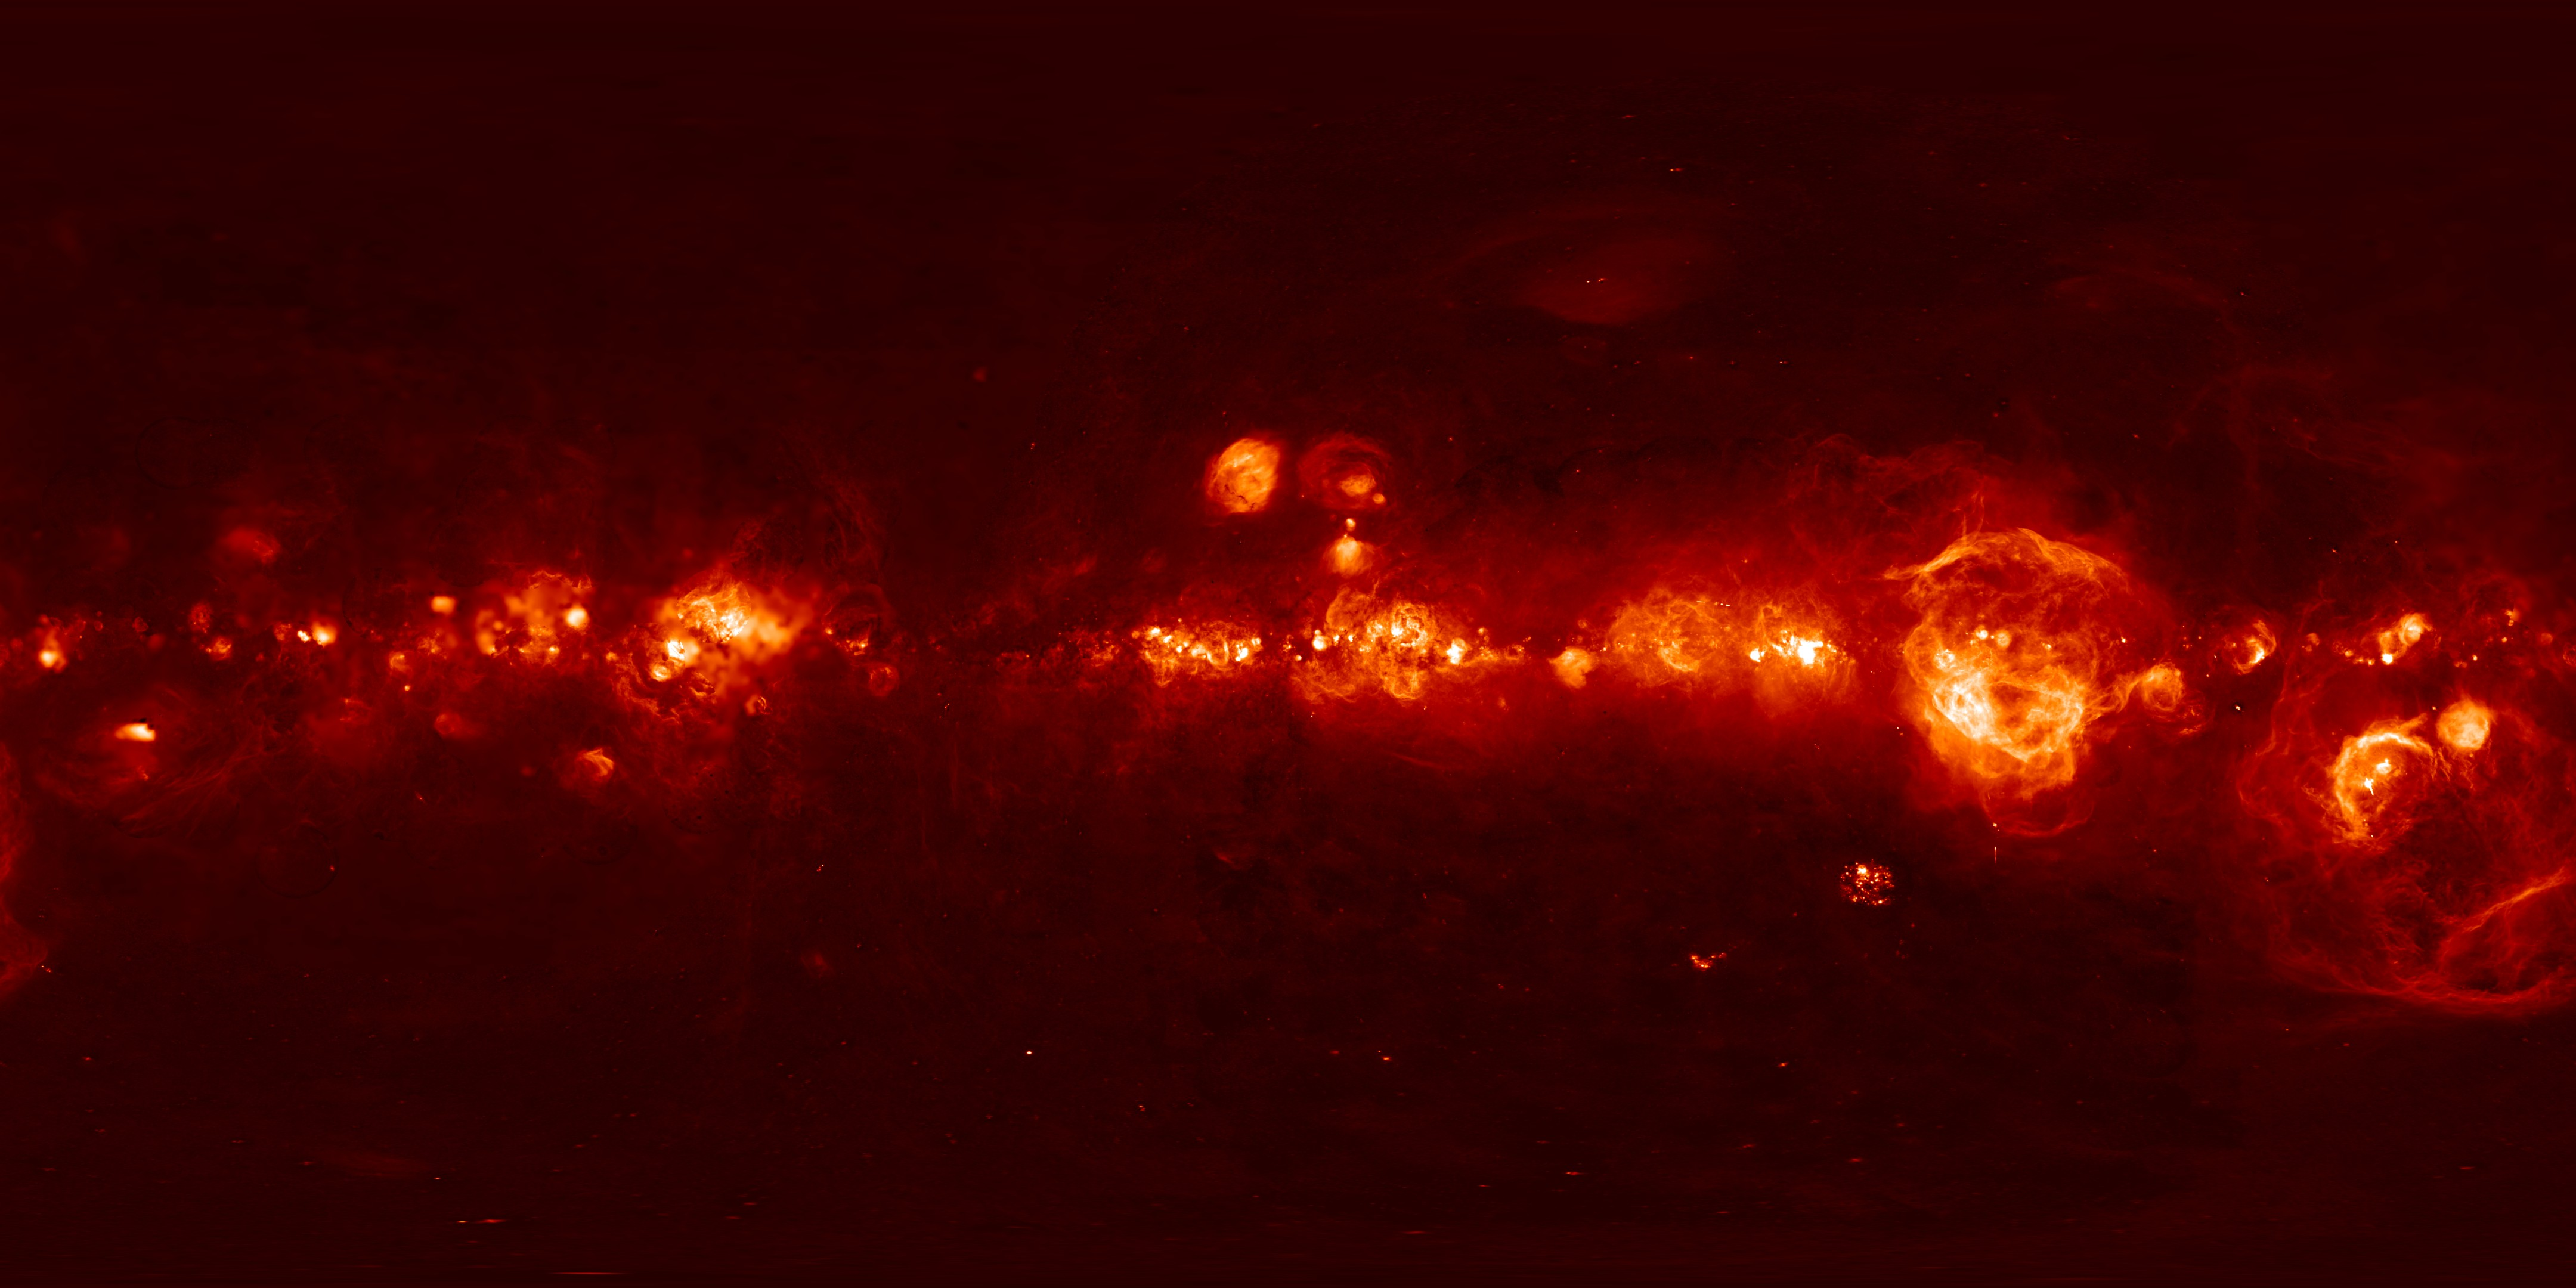
\includegraphics[width=1\linewidth]{../Document/Images/Ha}
\end{center}
	Εκπομπή Ha (\SI{656.28}{nm}) από συνδυασμό τριών διαφορετικών παρατηρήσεων (WHAM - VTSS - SHASSA) \cite{finkbeiner_2003}. 
	%Η εκπομπή Ha  προέρχεται από την επανασύνδεση ιονισμένων ατόμων υδρογόνου κοντά σε θερμούς αστέρες O και B (\ce{HII} Regions).
\end{frame}

\begin{frame}{Ψυχρή Μεσοαστρική Ύλη}
\begin{center}
	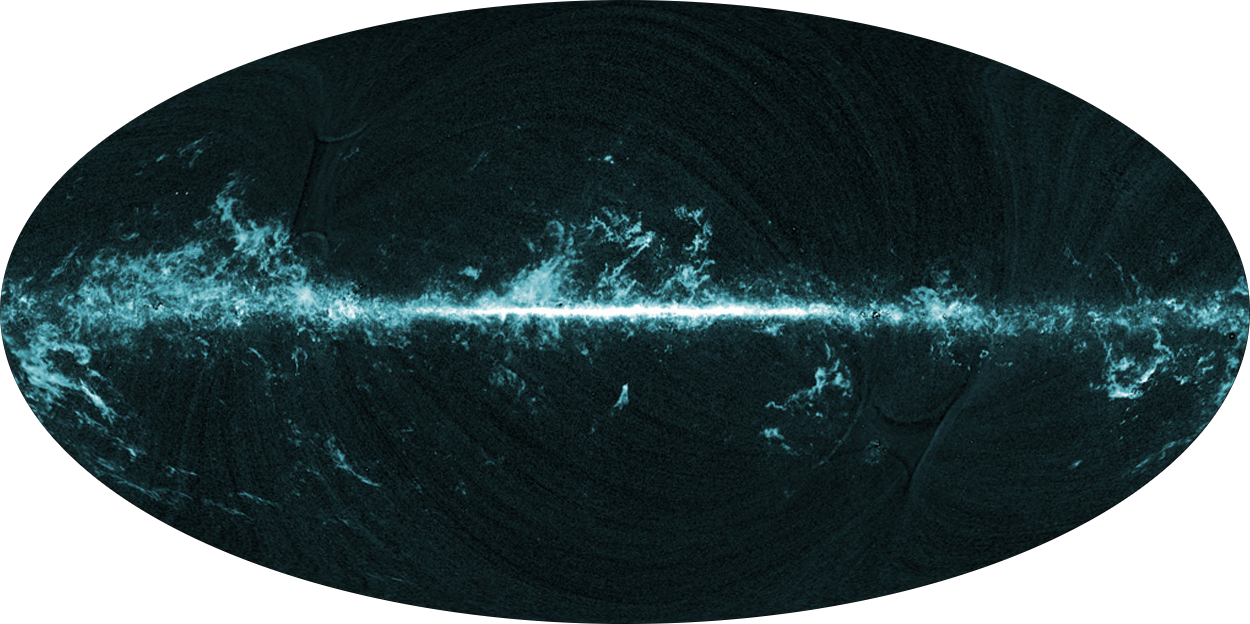
\includegraphics[width=1\linewidth]{../Document/Images/CO}
\end{center}
 Εκπομπή \ce{CO} που αντιστοιχεί σε θερμοκρασία \SI{5.5}{K} και αποδίδει ένα ραδιοφωνικό φωτόνιο στα \SI{2.6}{mm}.
\end{frame}

\begin{frame}{Μεσοαστρική Ύλη}{Φυσικά Χαρακτηριστικά - Σύνοψη}
\begin{table}
	\begin{tabular}{p{2.5cm} c  c  c }
		\toprule
		\multirow{2}{*}{Κατηγορία}  & Θερμοκρασία & Πυκνότητα   \\ 
		& \si{(K)} & \si{(cm^{-1})}  \\
		\midrule
		Μοριακά Νέφη & 10-50 & \num{>1e3} \\
		Ψυχρά Νέφη \ce{HI}  & \num{100} & \num{30} \\
		Θερμό \ce{HI}  & \num{1e3} & \num{0.1} \\
		Θερμό \ce{HII}  & \num{1e4} & \num{1e-2} \\
		Περιοχές \ce{HII} &  \num{1e4} & \num{>100} \\
		Υπέρθερμο Ιονισμένο αέριο &  \numrange{1e6}{1e7} & \num{1e-3} \\
		\bottomrule
	\end{tabular}
\end{table}
\end{frame}

\subsection{Μοριακά Νέφη}

% You can reveal the parts of a slide one at a time
% with the \pause command:
\begin{frame}{Μοριακά Νέφη}
	\begin{itemize}
		\item{Περιοχές όπου η ψυχρή μεσοαστρική ύλη έχει πυκνότητες ικανοποιητικά μεγαλύτερες από τη μέση πυκνότητα του μεσοαστρικού υλικού ώστε η ιδιοβαρύτητα του νέφους να παίζει σημαντικό ρόλο στη δυναμική του.}
		\item{Κατά τη βαρυτική κατάρρευση το ΜΝ κατακρημνίζεται σε όλο και πιο συμπυκνωμένες δομές έως ότου η πυκνότητα και η μάζα σε μια τέτοια περιοχή είναι αρκετή ώστε να γεννηθούν νέοι αστέρες. }
		\item{Αποτελούνται κυρίως από μοριακό Υδρογόνο \ce{H2}}
	\end{itemize} 
	
%  \begin{itemize}
%  \item {
%    First item.
%    \pause % The slide will pause after showing the first item
%  }
%  \item {   
%    Second item.
%  }
%  % You can also specify when the content should appear
%  % by using <n->:
%  \item<3-> {
%    Third item.
%  }
%  \item<4-> {
%    Fourth item.
%  }
%  % or you can use the \uncover command to reveal general
%  % content (not just \items):
%  \item<5-> {
%    Fifth item. \uncover<6->{Extra text in the fifth item.}
%  }
%  \end{itemize}
\end{frame}

\section{Second Main Section}

\subsection{Another Subsection}

\begin{frame}{Blocks}
\begin{block}{Block Title}
You can also highlight sections of your presentation in a block, with it's own title
\end{block}
\begin{theorem}
There are separate environments for theorems, examples, definitions and proofs.
\end{theorem}
\begin{example}
Here is an example of an example block.
\end{example}
\end{frame}

% Placing a * after \section means it will not show in the
% outline or table of contents.
\section*{Summary}

\begin{frame}{Summary}
  \begin{itemize}
  \item
    The \alert{first main message} of your talk in one or two lines.
  \item
    The \alert{second main message} of your talk in one or two lines.
  \item
    Perhaps a \alert{third message}, but not more than that.
  \end{itemize}
  
  \begin{itemize}
  \item
    Outlook
    \begin{itemize}
    \item
      Something you haven't solved.
    \item
      Something else you haven't solved.
    \end{itemize}
  \end{itemize}
\end{frame}



% All of the following is optional and typically not needed. 
\appendix
\section<presentation>*{\appendixname}
\subsection<presentation>*{For Further Reading}

\begin{frame}[allowframebreaks]
  \frametitle<presentation>{For Further Reading}
    
  \begin{thebibliography}{10}
    
  \beamertemplatebookbibitems
  % Start with overview books.

  \bibitem{Author1990}
    A.~Author.
    \newblock {\em Handbook of Everything}.
    \newblock Some Press, 1990.
 
    
  \beamertemplatearticlebibitems
  % Followed by interesting articles. Keep the list short. 

  \bibitem{Someone2000}
    S.~Someone.
    \newblock On this and that.
    \newblock {\em Journal of This and That}, 2(1):50--100,
    2000.
  \end{thebibliography}
\end{frame}

\end{document}


